\chapter{Introduction}\label{ch:introduction}

In the digital age written text has become ubiquitous. % (TODO: cite?~\autocite{salar-mohtaj-babak-naderi-2022-overview})
% TODO: Examples for important written text: Websites, Online Messages like E-Mails, Newspapers, Government Authorities (distribute Information)

Today the ability to comprehend text is a necessary prerequisite to actively participate in society. % nowadays
This poses a challenge to people with communication impairments~\autocite{easyLanguageBook}.
In Germany, about 12\% of the population has difficulties to understand and write standard german because of reduced literacy~\autocite{schomacker2023data}.
Complicated texts can act as a barrier which prevents these people from taking part in everyday life~\autocite{easyLanguageBook}
% could lead to exclusion,

Several attempts have been made to create a type of written language that is more comprehensible and accessible.
The primary goal of such languages is to improve communication for a broad range of people with limited reading and writing skills.
This group includes people with communication impairments, people with dementia, language learners, \gls{illit} and older people with visual impairments~\autocite{easyLanguageBook}.

In German, two simplified languages have gained popularity in recent years: \enquote{Easy Language} and \enquote{Plain Language}.

%The simplified language has to be simple enough to be understood by everyone.
%At the same time it should not be impractical for people that are proficient in standard language.


\section{Easy Language}\label{sec:el}

\gls{el} is a type of simplified language that is regulated by a set of rules.
There are multiple guidelines published by different organizations that define those rules.
The most commonly used guideline is distributed by the \enquote{\gls{nls}}~\autocite{netzwerkLS, easyLanguageBook}.

The \gls{nls} was founded in 2006 and became an official association in 2013~\autocite{netzwerkHistory}.
The association aims to popularize and standardize \gls{el} in Germany.
All members are volunteers~\autocite{netzwerkGoals}.
Among others, the \gls{nls} includes the following people in their target group:
\begin{itemize}[noitemsep]
    \item people with learning difficulties
    \item people with the illness dementia
    \item people that are not proficient in German
    \item people with reduced reading abilities
\end{itemize}
The \gls{nls} intends that texts written in \gls{el} are verified by certified examiners.
Examiners are trained at the \gls{nls} and are usually people in the target group~\autocite{netzwerkPruef}.

\subsection{Rules and Recommendations}\label{subsec:el-rules}
The rules for \gls{el} fall into the categories \enquote{Words}, \enquote{Numbers and Symbols}, \enquote{Sentences}, \enquote{Content} and \enquote{Presentation and Images}.

Words are supposed to be simple.
Technical and foreign words should be avoided.
If difficult words are unavoidable, they have to be explained.
Once a word was introduced to describe a subject, that word should be used again when the subject is referred to.

\begin{figure}[htb]
    \begin{center}
        \colorbox{badred!20}{
            \begin{minipage}{0.6\textwidth}
                \fontfamily{pag}
                A car drove past me.\\
                It was very fast.\\
                The vehicle was red.
            \end{minipage}
        }
        \colorbox{goodgreen!20}{
            \begin{minipage}{0.6\textwidth}
                \fontfamily{pag}
                A car drove past me.\\
                It was very fast.\\
                The car was red.
            \end{minipage}
        }
    \end{center}
    \caption[Using the same word to refer to the same subject.]{Using the same word to refer to the same subject (bottom). Using synonyms can be confusing (top).}
    \label{fig:subject_ref}
\end{figure}
Shorter words are preferred over longer words.
If long words are necessary, they should be split with a hyphen character (e.g.\ \enquote{Bundes-Gleichstellungs-Gesetz} instead of \enquote{Bundesgleichstellungsgesetz}).
Additional rules for words are
\begin{itemize}[noitemsep]
    \item the avoidance of acronyms
    \item the use of active voice over passive voice
    \item avoidance of genitive and conjunctive
    \item reduced use of negation
\end{itemize}
Numbers and symbols are another aspect that is addressed by the \gls{nls}-guideline.
Numbers should be written in arabic numerals.
For many people digits are easier to read than the spelled out word (e.g.\ \enquote{5 horses} instead of \enquote{five horses}).#
Thus, smaller numbers are to be witten in digits.
Very large numbers are replaced by rough estimations (e.g.\ \enquote{Many People} instead of \enquote{14.795 People}).
The same goes for percentages.
If unusual symbols (e.g.\ §) are used they need to be explained.

The structure of sentences has a big impact on readability. % TODO: quelle?
In \gls{el} sentences are supposed to be short.
Every sentence should only include one statement.
After each sentence a new line is started.
Sentences with simple structures like \enquote{subject, verb, object} are preferred.
More complex sentences should be broken up in smaller pieces.
These smaller pieces do not necessarily need to form a complete sentence.
\begin{figure}[htb]
    \begin{center}
        \colorbox{badred!20}{
            \begin{minipage}{0.6\textwidth}
                \fontfamily{pag}
                Do you want to go swimming or watch a movie?
            \end{minipage}
        }
        \colorbox{goodgreen!20}{
            \begin{minipage}{0.6\textwidth}
                \fontfamily{pag}
                Do you want to go swimming? \\
                Or watch a movie?
            \end{minipage}
        }
    \end{center}
    \caption[Splitting longer sentences in \glsentrylong{el}.]{Splitting longer sentences in \glsentrylong{el}. To comply with the rules of \gls{el} the (top) sentence is split in two. The second part of the (bottom) example does not form a complete sentence on its own.}
    \label{fig:split_sentence}
\end{figure}
%\begin{mybox}{Bad example}
%    Do you want to go swimming? \\
%    Or watch a movie?
%\end{mybox}
Sentences with subordinate clauses can be broken up similarly.

Topics should not be distributed across the text.
Related content should be kept together.
References to other texts are to be avoided.
In the translation process from standard German to \gls{el} content can be omitted if necessary.
Likewise, additional content can be added to make the text more understandable.

The presentation of text is another aspect that impacts clarity and readability.
The \gls{el}-guideline recommends using a big font size and big line spacing.
Furthermore, text is to be left-aligned.
Backgrounds are supposed to be in light color while the written text is colored darkly.
Text should be structured in many paragraphs with frequent headlines.
Using bullet points instead of comma separated enumerations improves clarity.
Images can be added to accompany the text~\autocite{netzwerkLS}.

\subsection{Prevalence and Adoption of Easy Language}\label{subsec:el-adop}

\glsentrylong{el} contains features that go against standard german.
The unique layout with very short lines makes it easy to recognize texts in \gls{el}.
This helps the target group to find texts written in \gls{el} easily.
But the strong divergence from standard German has been repeatedly criticised.
In 2015, the Federal State Parliament of Schleswig-Holstein passed a law to make elections more accessible.
Information regarding elections was sent out to all voters in \gls{el}.
This sparked outrage in the population and was denounced by multiple politicians.
As a result the passed law was reverted~\autocite{easyLanguageBook}.

While \gls{el} has yet to find acceptance in the general population, it has already been incorporated into german law.
In 2002 the \gls{bgg} was adopted.
The \gls{bgg} guarantees equal living conditions to people regardless of disabilities.
In 2018 the \gls{bgg} was extended to include clearer instructions for accessibility~\autocite{bggInfo}.
Since then, public authorities have to provide information in \gls{el} as specified in section 2, paragraph 11~\autocite{bgg2018}.
Today \gls{el} can be found on many websites of government departments and municipal institutions (e.g.\ the City Cologne: \url{https://www.stadt-koeln.de/artikel/07808/index.html}).

\begin{figure}
    \centering
    \colorbox{goodgreen!20}{
        \begin{minipage}{0.6\textwidth}
            Fische sind Tiere. \\
            Sie leben im Wasser. \\
            In Flüssen, im Meer und in Seen. \\
            \\
            Fische atmen durch Kiemen. \\
            Das ist ein Körper-teil. \\
            Dadurch können sie unter Wasser atmen.
        \end{minipage}
    }
    \caption[Text written in \glsentrylong{el}.]{Text written in \gls{el} taken from the online dictionary \enquote{Hurraki} (\url{https://hurraki.de/wiki/Fische}).}
    \label{fig:easy_text}
\end{figure}


\section{Plain Language}\label{sec:pl}
\gls{pl} is a simplified language that is much closer to standard language.
Originally, it was not intended for people with disabilities.
\gls{pl} is often used to explain domain-specific texts in expert language to less informed people.
Moreover, it addresses language learners, e.g.\ migrants and people that learn German as a second language~\autocite{easyLanguageBook}.

In the English language guidelines for \gls{pl} have existed for a long time.
Some early works on more accessible language were published in the beginning of the 20th century.
From the 1960s on the US government pushed to propagate the use of \gls{pl}.
The goal was to improve communication between citizens and experts from administrative institutions.
Several instruction manuals for \gls{pl} were distributed.
Since 2010 federal agencies in the US are required to offer information in a form that is well understood by the citizens.

In Germany efforts for \gls{pl} have only been made very recently.
In the 1980s \enquote{Bürgernahe Sprache} (in English: \enquote{language that is close to the citizens}) was created to make administrative texts more comprehensible.
\enquote{Bürgernahe Sprache} does not take people with communication impairments and less educated people into account.
Thus, it does not satisfy all expected conditions of a simplified language.
In the 2000s multiple approaches for \gls{pl} with a broader target groups were attempted.
But none of them have been widely accepted as a standard yet.
Typical features of \gls{pl} are
\begin{itemize}[noitemsep]
    \item use of common words
    \item use of short words
    \item avoidance of ambiguous words
    \item precise formulations
    \item short sentences
    \item active voice
    \item clear sentence structure (e.g.\ a maximum of two subordinate clauses)
    \item avoidance of acronyms
\end{itemize}
These directives are similar to some rules in the \gls{el}-guideline.
But \gls{pl} does not break any rules of standard German.
That might be a reason why \gls{pl} is generally viewed in a more positive light than \gls{el} by many people. % viewed favorably
Moreover, \gls{pl} can be more flexible and less restrictive as there are no fixed rules.
Writers of \gls{pl} are supposed to factor in the audience of the text and make changes accordingly~\autocite{easyLanguageBook}.

\begin{figure}
    \centering
    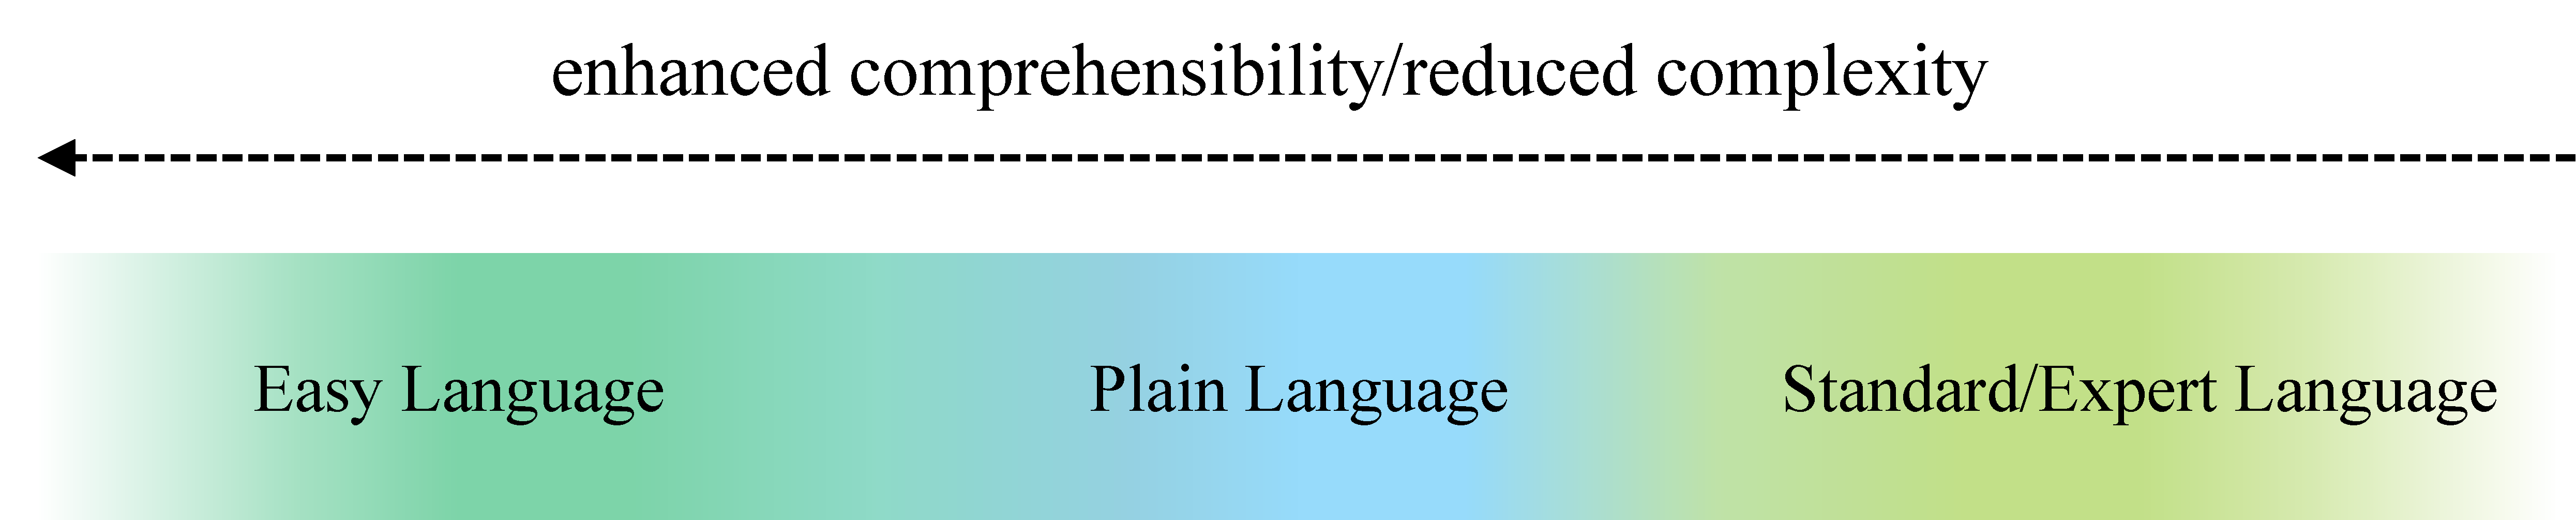
\includegraphics[width=\linewidth]{images/easy_languages}
    \caption[Different levels of text complexity and comprehensibility.]{Different levels of text complexity and comprehensibility. The different types of languages overlap in certain aspects~\autocite{easyLanguageBook, selbsterstellt}}
    \label{fig:languages}
\end{figure}


 % TODO: CEFR, UN, (BITV 2.0)
%\section{Terminologie}\label{sec:term}

%ambiguity of terminology

%    more difficult to understand than easy language
%
%
%From~\autocite{un2008}:
%Article 9 -Accessibility: "sinage in easy to read and understand forms", "ensure access to information"
%
%Article 2: plain-language listed under communication
%
%Article 29 - Participation in political and public life

%easy, plain, simple with very similar meanings

%    different guidelines:
%        inclusion europe
%        Netzwerk Leichte Sprache -> most commonly used
%        Barrierefreie-Informationstechnik-Verordnung (BITV 2.0)
%
%    rulebooks published by Duden


%

%From~\autocite{schomacker2023data}:
%"Easy language is roughly equivalent with level A2 of the Common European Framework of Reference for Languages (CEFR)"

\section{Automatic Language Simplification}\label{sec:langSimp}

Writing texts in \gls{pl} or \gls{el} and translating complex texts into simpler forms requires much effort~\autocite{easyLanguageBook}.
Hence, there is a demand for tools that can assist in this process.
In the context of \gls{nlp} the task of computer aided reduction of text complexity is known as \gls{ats}~\autocite{Ansch_tz_2023}.
The goal of \gls{ats} is to create a system that takes a text in standard or expert language as an input and outputs a simplified version of that text.
\gls{ats} is similar to other \gls{nlp}-tasks like summarization~\autocite{rios-etal-2021-new} and language translation~\autocite{aumiller2022klexikon}.
It is a \gls{seq2seq}-task~\autocite{Ansch_tz_2023} meaning the desired system has to processes and output texts of varying lengths.
\gls{ats} is a relatively new \gls{nlp}-task~\autocite{schomacker2023data}.
Especially simplification of German text has not seen a lot of research~\autocite{Ansch_tz_2023}.

Some \gls{ats}-methods focus only on sentence-level simplifications while other approaches aim to simplify whole documents.
Simplifications on sentence-level have the advantage that the \gls{ats}-System has to perform less complex transformations on the text.
But certain features of \gls{el} like the organization of content order and structure (see section~\ref{subsec:el-rules}) cannot be taken into account. %TODO: Braucht das eine quelle oder ist das offensichtlich?
Document-level simplifications do not have this problem.
However, they require the \gls{ats}-system to be able to process longer sequences and to carry out very complex modifications.

An early rule-based approach for language simplification into \gls{el} was presented by~\autocite{suter2016}.
This approach employed dictionaries to substitute difficult symbols.
Sentences and long words were split through a defined rule-set and additional explanations were added by inserting entries from the online dictionary \enquote{Hurraki}.
~\autocite{Garain2019} created another rule-based method using parse-trees to simplify english sentences.

Solutions based on \enquote{Deep Learning} are generally superior to rule-based methods for language translation tasks.
However, they require vast amounts of data~\autocite{otter2019survey}.
The data is usually a collection of texts (known as a \enquote{corpus}) which are related to the task at hand.
In the setting of language translation \enquote{parallel data} is very useful.
A parallel corpus contains pairs of source and target texts that function as an example for the task.
For \gls{ats} a parallel example would consist of a source text in standard language and a corresponding simplification.
Creating a parallel corpus is difficult as source and target text need to be properly aligned.
It is much easier to assemble a monolingual corpus that usually only contains texts in the target language~\autocite{chan2023routledge}.
While these monolingual corpora are less optimal than parallel data they can still be used in various ways to improve machine translation systems~\autocite{lample2018unsupervised, burlot2019using, chan2023routledge}.

Unfortunately, data for german language simplification is scarce~\autocite{Ansch_tz_2023}.
Most recent research has focused on creating corpora for \gls{el} and \gls{pl} to make Deep Learning approaches more feasible.

\textcite{klaper-etal-2013-building} build the first parallel corpus for german text simplification that consists of 256 texts~\autocite{ebeling2022}.
This corpus was later extended by~\textcite{battisti-etal-2020-corpus}.
The texts were extracted from PDF files and websites.
The extended corpus includes 6,217 documents of which the majority are monolingual (i.e.\ simplifications only) and is referred to as the \enquote{Web-Corpus} by~\textcite{ebeling2022}.
\textcite{sauberli-etal-2020-benchmarking} gather parallel data from news items provided by the \enquote{Austria Presse Agentur} (APA) that were manually simplified under the guidelines of \gls{capito}.
All in all the \enquote{APA-Corpus} contains 2,426 distinct documents~\autocite{ebeling2022}.
The data is then used to train \gls{ats}-models for sentence-level simplifications using the transformer architecture (see section~\ref{sec:trans}). %TODO: first neural simplification approach based on transformers, "lack of fluency and content preservation" (~\autocite{Ansch_tz_2023})
This is possibly the first transformer-based approach to german \gls{ats}~\autocite{Ansch_tz_2023}.
The company \gls{capito} also built a parallel corpus of about 1000 documents that is not publicly available~\autocite{ebeling2022}.

All the above-mentioned datasets contain a mix of different simplification levels.
Moreover, due to copyright issues, most of the data is not easily accessible~\autocite{stodden-etal-2023-deplain}.

\textcite{rios-etal-2021-new} create and publish a parallel document-level corpus from articles of the Swiss news magazine \enquote{20 Minuten} containing 17,905 article pairs.
The simplifications are written in \gls{pl} and are strongly summarized.
They train transformer-based language models on the published dataset while also including the \enquote{Capito Corpus} and the \enquote{APA Corpus}.

Another transformer-based approach for \gls{ats} is presented by~\textcite{spring-etal-2021-exploring}.
Their models are also trained on the corpora \enquote{Capito} and \enquote{APA} and can output different levels of simplified language based on the \gls{cefr}.

\textcite{aumiller2022klexikon} align entries from the German children’s encyclopedia \enquote{Klexikon} with Wikipedia articles in standard language.
This method explores the task of simultaneous simplification and summarization, as the Klexikon articles are usually much shorter than their Wikipedia counterparts.

Current publicly available \gls{llm} are capable of completing a vast number of different tasks.
\textcite{deilen2023using} test the feasibility of using ChatGPT-3.5 as an \gls{ats}-system.
They try different prompt strategies to translate text into \gls{el}.
But while outputs are easier to understand, they are missing information and do not follow the rules of \gls{el}.

\textcite{toborek2023new} experiment with automatic sentence alignment of parallel documents.
They publish corpus of 708 aligned documents by providing \gls{webscraper}s for different websites.

To overcome the aforementioned scarcity of parallel data~\textcite{Ansch_tz_2023} use monolingual \gls{el}-data to pretrain \gls{causal-lm}s.
The pretrained models output text in the style of \gls{el} and show improved capabilities in the \gls{ats}-downstream-task.
They publish the \gls{webscraper}s that were used to gather the monolingual data\footnote{\url{https://github.com/brjezierski/scrapers}}.
Running those scrapers yields more than 20,000 documents in either \gls{el} or \gls{pl}.
%training ATS task on pretrained mBart model (replacing decoder with above-mentioned GPT-like Decoders, trainig cross-attention only)

\textcite{stodden-etal-2023-deplain} address issues with current datasets for german \gls{ats} and provide a new parallel corpus that is more accessible than previous corpora.
It is called \enquote{DEPlain} and contains about 1,000 parallel documents (either in \gls{el} or \gls{pl}) of which parts ca be downloaded directly from the internet\footnote{\url{https://github.com/rstodden/DEPlain}}, scraped with a provided script\footnote{\url{https://github.com/rstodden/data_collection_german_simplification}} and be directly requested from the authors.
The corpus contains documents from the Austria Presse Agentur (APA) so it might overlap with the APA Corpus.

Another small dataset is provided by \textcite{naderi2019subjective}.
It consists of 250 parallel sentence-level simplifications in \gls{pl} and was originally used in the context of text complexity assessment.

%\enquote{Deep Learning} is a subset of \enquote{Machine Learning}~\autocite{jagdaleDeepLearning2022}.

\subsection{Previous Work}\label{subsec:previous-work}

In a previous work~\textcite{klöser2024german} extend the scrapers of~\textcite{Ansch_tz_2023} to gather monolingual texts in \gls{el} and \gls{pl}.
By prompting ChatGPT to generate corresponding texts in standard language, semi-synthetic text pairs are formed.
To encourage variation in the generated text, 15 distinct prompts are used.
The newly formed parallel corpus is then used to train language models on the task of document-level \gls{ats}.
This process is sometimes referred to as \enquote{back-translation}~\autocite{sennrich-etal-2016-improving}.

The trained models are evaluated by applying three different metrics that compare reference simplifications to model outputs.
A closer inspection of these metrics shows that rule-based evaluations for \gls{el} are limited and further research on this topic is needed.
Manual evaluation of simplifications reveals that

While the results of the trained models are promising, there is still a lot of room for improvement.
\begin{itemize}[noitemsep]
    \item The models have difficulties simplifying short texts (i.e.\ simplifications on sentence-level).
    \item Topics and domains of the training documents were mainly news items, dictionarys or informative texts.
    \gls{generalization} to other domains (e.g.\ fiction or law) is subpar.
    \item There is a certain bias towards texts generated by ChatGPT.
    Simplifications of naturally written texts work well, but are quite different from simplified ChatGPT texts.
    \item Simplifications are very linear in the way that they often align with the content order of their original documents.
    Reorganization of content as encouraged by \gls{el} is rare.
    \item Some model outputs can contain very obvious mistakes that result in nonsensical sentences.
    This possibly results from the limited capabilities of the used base model and architecture.
\end{itemize}

The goal of this work is to improve the aforementioned models by extending the training data and testing different model architectures and training methods.


% TODO: Evaluation
%From~\autocite{madina2023easytoread} TODO: Survey
%From~\autocite{salar-mohtaj-babak-naderi-2022-overview}: TextComplexity 2022
%
%BLEU: ~\autocite{papineni-etal-2002-bleu}
%SARI: ~\autocite{xu-etal-2016-optimizing}
%METEOR: ~\autocite{banerjee-lavie-2005-meteor}
